% =====================================================================
\chapter{Técnicas de Ciencia de Datos}
\label{cap:tecnicas}

La ciencia de datos combina programación, estadística y conocimiento del dominio para
extraer conocimiento de datos. Este trabajo siguió las fases del proceso CRISP-DM
\citep{wirth2000crispdm}: comprensión del problema (capítulos~\ref{cap:objetivos}
y~\ref{cap:marco}), comprensión y preparación de los datos, modelado y evaluación
(capítulos~\ref{cap:desarrollo} y~\ref{cap:resultados}). Todo se programó en Python; los
modelos estadísticos usan la librería \texttt{statsmodels} \citep{seabold2010} y los de
lenguaje, \texttt{transformers} y \texttt{spaCy}. La figura~\ref{fig:mapa} resume el
\textit{pipeline} completo, con el resultado de cada paso.

\begin{figure}[H]
\centering
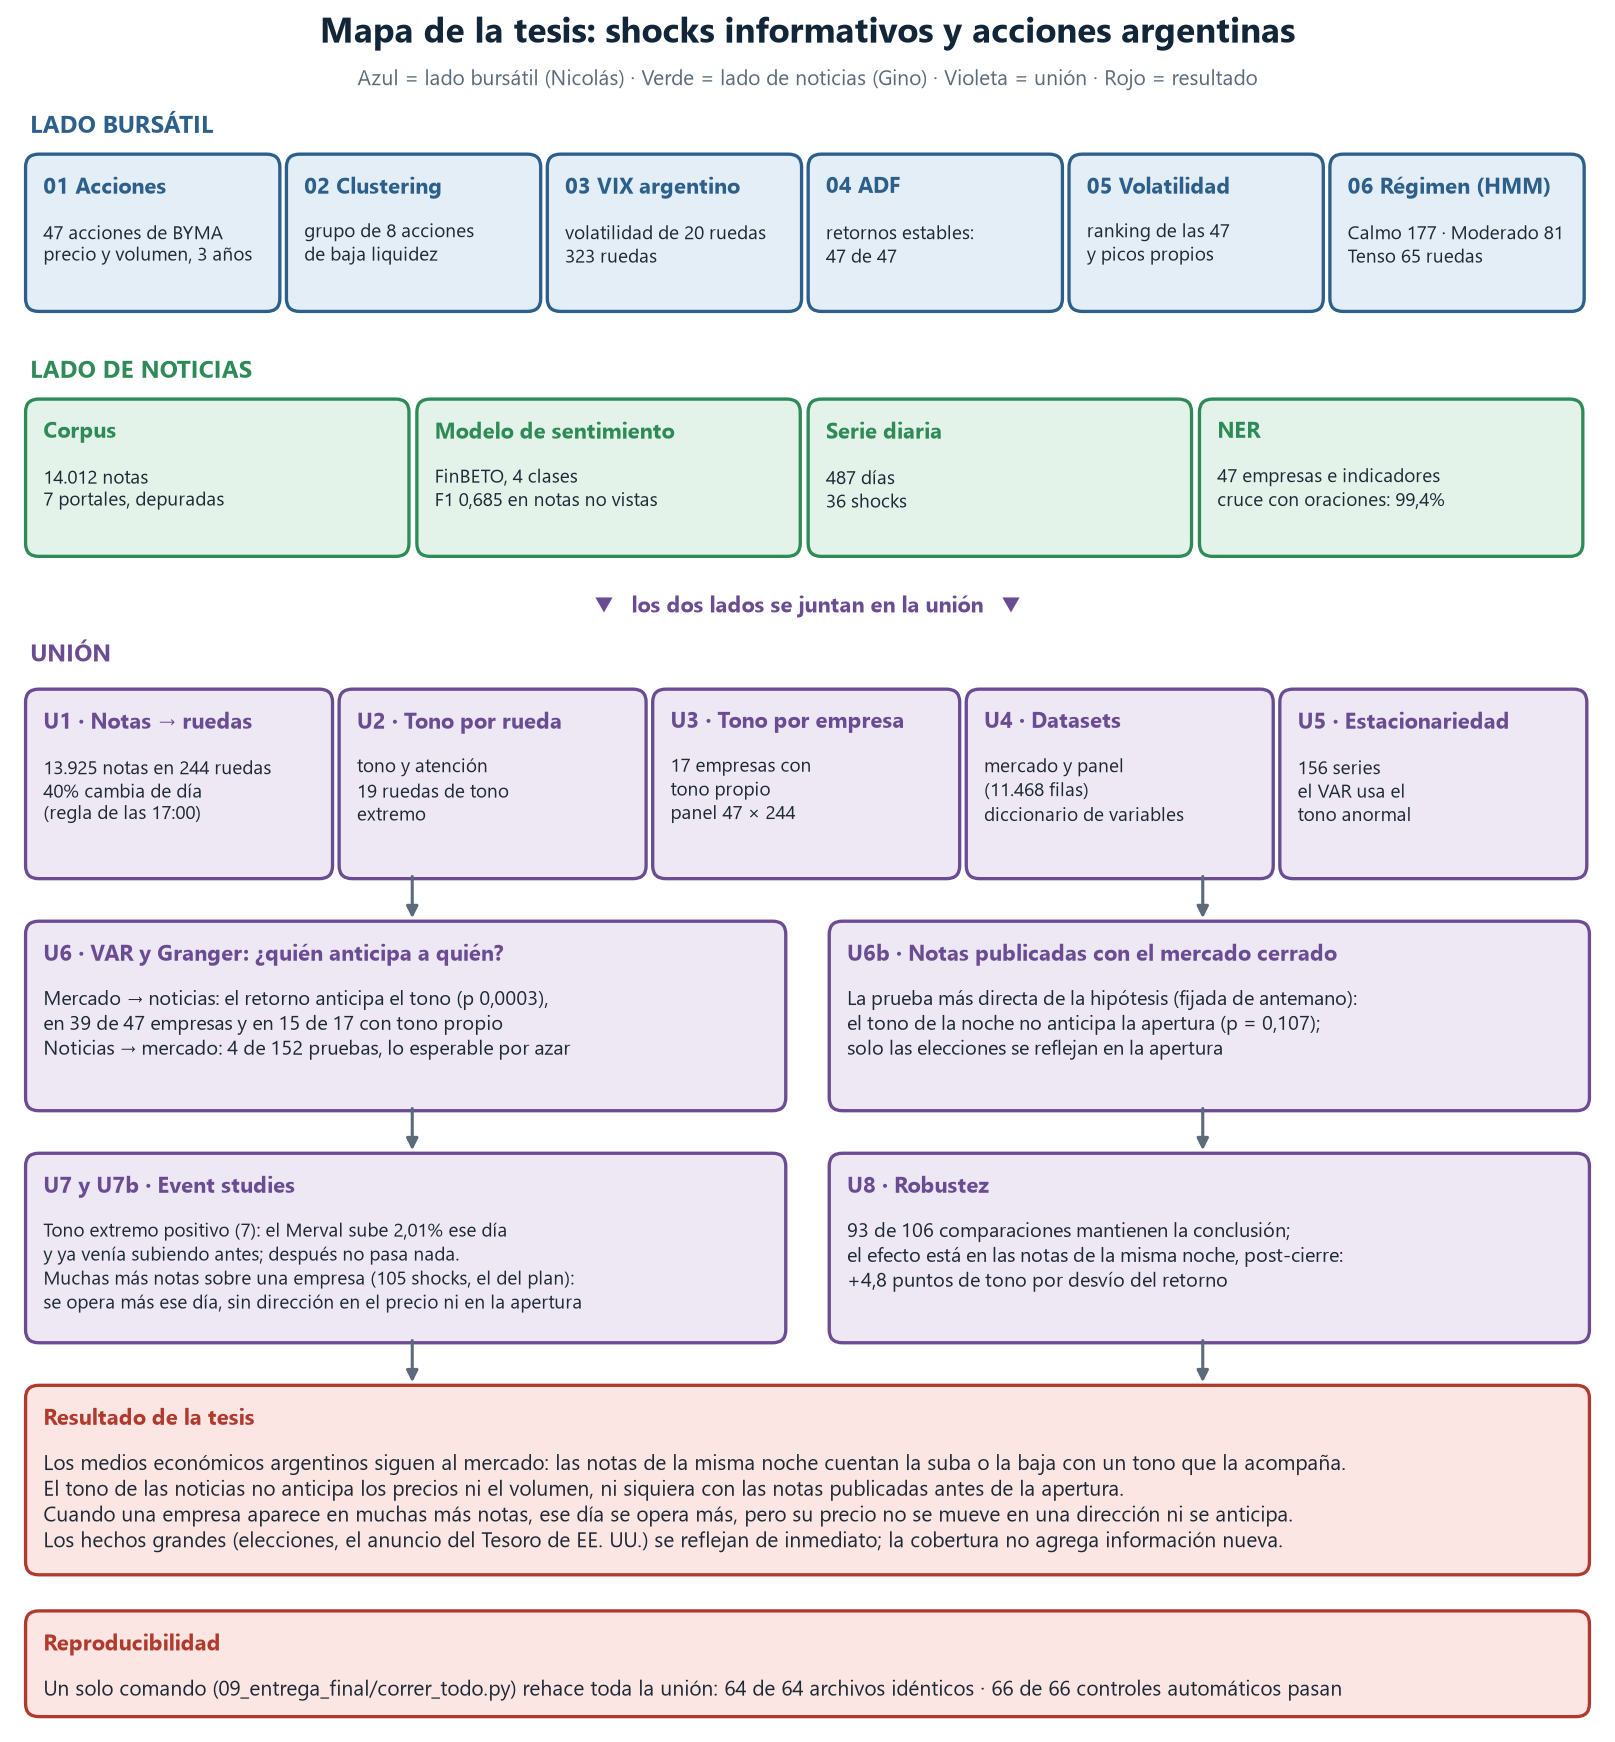
\includegraphics[width=0.93\linewidth]{mapa_tesis.png}
\caption{Mapa de la tesina: el lado bursátil (azul), el lado de noticias (verde), la unión
(violeta) y el resultado (rojo). Fuente: elaboración propia
(\carpeta{Unión/09_entrega_final/mapa_tesis.py}, que lee los resultados de cada carpeta).}
\label{fig:mapa}
\end{figure}

% ---------------------------------------------------------------------
\section{Adquisición de datos}
\label{sec:tec-adquisicion}

\subsection{Web scraping de noticias}

El \textit{web scraping} es la extracción automática de información de páginas web. Para un
corpus histórico de noticias hay dos caminos. El primero es Internet Archive: su
\textit{Wayback Machine} guarda capturas de millones de páginas y su API CDX permite listar
las capturas de un sitio en un rango de fechas; así se puede reconstruir una ventana más larga
que la que exponen los propios portales, a costa de depender de qué capturó un tercero
\citep{garg2025wayback}. El segundo son los \textit{mapas del sitio} (\texttt{sitemap.xml}),
que los portales publican para los buscadores y que listan sus notas recientes. Una vez
obtenida la página, hay que separar el texto de la nota del «relleno» (menús, publicidad,
firmas) y extraer sus metadatos (título, fecha, autor). Se usó una estrategia en capas: los
datos estructurados JSON-LD primero, después las metaetiquetas Open Graph, el título
\texttt{<h1>}, la librería \texttt{trafilatura} \citep{barbaresi2021} y, como último recurso,
reglas sobre el HTML con BeautifulSoup. Las herramientas de extracción de contenido fallan con
frecuencia en el relleno y en los metadatos \citep{foley2026wcxb,hatwar2024author}, por lo
que un corpus web tiene que auditarse antes de usarse: buscar plantillas, duplicados y
contenido que no corresponde \citep{dodge2021c4}. Los duplicados, además, distorsionan
cualquier modelo que se entrene con ese texto \citep{lee2021dedup}. Como fuente alternativa
para ampliar un corpus de noticias, \citet{fronzetti2026gdelt} reconstruyen el texto completo
de notas a partir de la base GDELT.

\subsection{Precios de acciones}

Los precios diarios (apertura, máximo, mínimo, cierre y volumen) se descargaron de Yahoo
Finance con la librería \texttt{yfinance}, para cada acción (\texttt{TICKER.BA}) y para el
índice (\texttt{\^{}MERV}). Yahoo entrega precios ajustados por divisiones y dividendos en
acciones, pero tiene tres problemas conocidos que se trataron en la limpieza: agrega filas
«fantasma» en los feriados, falla de forma intermitente para algunos tickers y, en algunos
casos, aplica mal los ajustes por eventos corporativos.

% ---------------------------------------------------------------------
\section{Análisis exploratorio de series de tiempo}
\label{sec:tec-eda}

\subsection{Estacionariedad: ADF y KPSS}

Un VAR necesita series estacionarias, que oscilen alrededor de un nivel estable. Si se usan
series con tendencia, dos variables que suben juntas parecen relacionadas aunque no lo estén.
La prueba de Dickey-Fuller aumentada \citep[ADF;][]{dickey1979} tiene como hipótesis nula que
la serie tiene raíz unitaria (no es estacionaria); un p-valor menor a 0,05 permite rechazarla.
La prueba KPSS \citep{kpss1992} hace la pregunta al revés: parte de suponer que la serie es
estacionaria y busca evidencia en contra. Usadas juntas dan cuatro resultados posibles
(tabla~\ref{tab:adf-kpss}). Los rezagos del ADF se eligen con el criterio de Akaike.

\begin{table}[H]
\centering\small
\begin{tabular}{@{}llL{6.3cm}@{}}
\toprule
\textbf{ADF} & \textbf{KPSS} & \textbf{Conclusión} \\
\midrule
Rechaza la raíz unitaria & No rechaza la estacionariedad & Estacionaria \\
Rechaza la raíz unitaria & Rechaza la estacionariedad & Estacionaria con memoria (persistente) \\
No rechaza & No rechaza & Inconclusa: los datos no alcanzan para decidir \\
No rechaza & Rechaza & No estacionaria \\
\bottomrule
\end{tabular}
\caption{Lectura conjunta de las pruebas ADF y KPSS. Fuente: elaboración propia.}
\label{tab:adf-kpss}
\end{table}

\subsection{Volatilidad realizada}

La volatilidad realizada de un activo en el día $t$ es el desvío estándar de sus retornos
diarios en las últimas 20 ruedas, anualizado:
\begin{equation}
\sigma_t = \sqrt{252}\cdot \operatorname{desv}\left(r_{t-19},\dots,r_t\right)\cdot 100,
\qquad r_t = \frac{P_t - P_{t-1}}{P_{t-1}}.
\end{equation}
Aplicada al índice da el VIX argentino; aplicada a cada acción, su volatilidad propia. El
factor $\sqrt{252}$ es la convención internacional de ruedas por año. BYMA tiene unas 244
ruedas por año por sus feriados; usar ese número bajaría todos los valores un 1,5\%, sin
cambiar ninguna comparación. La volatilidad de las acciones individuales tiene además un
componente común entre empresas \citep{kalnina2024}.

\subsection{Clustering de acciones}

El clustering agrupa elementos parecidos sin etiquetas previas. Para series financieras, la
distancia habitual entre dos acciones es $1-\rho$, donde $\rho$ es la correlación de sus
retornos \citep{mantegna1999,marti2021}. Se usaron tres algoritmos: K-Means, que forma $k$
grupos minimizando la distancia de cada elemento al centro de su grupo; el jerárquico, que va
uniendo los elementos más cercanos; y el árbol de expansión mínima (MST), que conecta todas
las acciones con la menor distancia total y que en los mercados tiende a agrupar por sector
\citep{mantegna1999,onnela2003}. La cantidad de grupos se eligió con el índice de silueta
\citep{rousseeuw1987}, que compara para cada elemento qué tan cerca está de su propio grupo y
qué tan lejos del más cercano. El clustering de acciones se aplicó en mercados emergentes de
tamaño comparable \citep{ghosh2025,ramirez2025,alexandre2021}, y se sabe que los grupos
cambian entre períodos \citep{arratia2013,pharasi2020}.

La liquidez es un problema central para estas técnicas. Cuando una acción no opera, Yahoo
Finance repite el precio del día anterior con volumen cero. Esos días de precio «quieto»
bajan artificialmente la correlación medida con las demás acciones
\citep{nanyonga2025,busca2023} y pueden generar adelantos y retrasos espurios entre acciones
\citep{lomackinlay1990,huth2011}. La frecuencia de días sin movimiento es, de hecho, una
medida clásica de iliquidez \citep{lesmond1999}.

\subsection{Regímenes de mercado}

Un modelo de cambio de régimen de Markov supone que la serie (aquí, el VIX argentino) tiene
una media y una varianza distintas en cada uno de $k$ estados ocultos, y que el mercado pasa de
un estado a otro según una matriz de probabilidades de transición
\citep{hamilton1989,kim1994}. En la literatura de mercados se lo suele llamar HMM
\citep{rabiner1989}. Se estimó con \texttt{MarkovRegression} de \texttt{statsmodels} para
$k=2$ a 6 y se eligió $k$ por el criterio bayesiano de información \citep[BIC;][]{schwarz1978},
descartando los ajustes que no convergen o que crean un régimen de menos de cinco días
(estados degenerados, una falla conocida de los modelos de mezcla). A cada día se le asigna el
régimen de mayor probabilidad \textit{suavizada}, que usa toda la serie; se guarda también la
versión \textit{filtrada}, que solo usa la información disponible hasta ese día y es la
adecuada si el régimen se usa para pronosticar \citep{majumder2023}.

% ---------------------------------------------------------------------
\section{Modelos de lenguaje}
\label{sec:tec-lenguaje}

\subsection{FinBETO: BETO adaptado al dominio}

BERT \citep{devlin2019bert} es un modelo de lenguaje preentrenado con la tarea de adivinar
palabras ocultas en un texto (\textit{masked language modeling}, MLM). BETO es su versión
entrenada en español \citep{canete2020beto}. Para clasificar sentimiento se le agrega una capa
de salida y se lo ajusta con oraciones etiquetadas (\textit{fine-tuning}), como hizo FinBERT
en inglés \citep{araci2019finbert}. Antes del ajuste, conviene seguir el preentrenamiento con
texto del propio dominio, porque mejora el desempeño en la tarea final
\citep{gururangan2020dapt}. FinBETO es el resultado de los dos pasos sobre la prensa económica
argentina.

Para el ajuste fino hacen falta oraciones etiquetadas, y no existía un conjunto público de
prensa económica argentina. Se usó un modelo de lenguaje como etiquetador, una práctica que
puede igualar o superar a anotadores contratados \citep{gilardi2023chatgpt} y que también se
evaluó en textos financieros \citep{aguda2024llmannot}. El etiquetador fue Gemma
\citep{gemma2026gemma4}, ejecutado localmente. La condición para que esa práctica sea válida
es contrastar el modelo con anotadores humanos en una muestra; \citet{calderon2025alttest}
proponen una prueba estadística para hacerlo con pocas oraciones.

La evaluación tiene una trampa conocida: la \textit{fuga de información}
(\textit{leakage}), cuando datos de prueba también están, total o parcialmente, en el
entrenamiento, lo que infla los resultados \citep{kapoor2023leakage}. Con noticias, la forma de
dividir los datos cambia mucho el resultado \citep{xue2026temporal}. La métrica principal es
el F1 macro: el promedio simple del F1 de cada clase, que no premia acertar solo la clase más
frecuente. El modelo de referencia fue \texttt{finiteautomata/beto-sentiment-analysis}, de la
librería pysentimiento \citep{perez2021pysentimiento}, un BETO ajustado con tuits.

\subsection{Reconocimiento de entidades nombradas}

El reconocimiento de entidades nombradas (NER) identifica en un texto los nombres de
personas, organizaciones, lugares y otras entidades. Los cuatro tipos que usan los modelos en
español (PER, ORG, LOC y MISC) vienen de la tarea compartida CoNLL-2002
\citep{tjongkimsang2002conll}. Se usó el modelo \texttt{es\_core\_news\_lg} de spaCy
\citep{honnibal2020spacy}, combinado con un \textit{gazetteer}: un diccionario curado de
nombres que se buscan literalmente en el texto y se unen a un identificador único, como se
hace en otros dominios \citep{ujiie2021dict}. Las alternativas con modelos de lenguaje como
etiquetadores \citep{golde2025finerweb} y la detección de las entidades centrales de una nota
\citep{asgarieh2024salient} quedan como mejoras posibles.

% ---------------------------------------------------------------------
\section{Modelos de series de tiempo y pruebas}
\label{sec:tec-modelos}

\subsection{VAR, causalidad de Granger e impulso-respuesta}

Un VAR con $p$ rezagos explica el vector de variables de hoy, $y_t$, con sus valores de las
$p$ ruedas anteriores:
\begin{equation}
y_t = c + A_1\, y_{t-1} + A_2\, y_{t-2} + \dots + A_p\, y_{t-p} + \varepsilon_t .
\end{equation}
En el VAR del mercado, por ejemplo, $y_t$ contiene el tono anormal de las noticias, la
atención anormal, el retorno del S\&P~Merval y el monto operado anormal. Los rezagos se eligen
entre 1 y 5 con el criterio de Akaike \citep{lutkepohl2005}. La prueba de Granger de
«tono \flecha{} retorno» es una prueba $F$ de que todos los coeficientes del tono rezagado en
la ecuación del retorno valen cero \citep{granger1969}: si se rechaza, el pasado del tono ayuda
a anticipar el retorno. La función de impulso-respuesta muestra cómo responde cada variable,
rueda a rueda, a un golpe de un desvío en otra; su banda del 95\% indica si la respuesta es
distinta de cero. Para ordenar el golpe dentro de una misma rueda, las noticias van primero,
porque el precio de una rueda no puede cambiar una nota ya publicada.

\subsection{Estudio de eventos}

En el estudio de eventos, la rueda del evento es la 0. El retorno normal se estima en la
ventana $[-25,-4]$, que termina antes del evento para que no contamine su propia comparación,
y el retorno anormal se mide en $[-3,+5]$ \citep{mackinlay1997}. Para una acción se usa el
modelo de mercado:
\begin{equation}
RA_{i,t} = r_{i,t} - \left(\hat\alpha_i + \hat\beta_i\, r_{M,t}\right),
\qquad CAR_i[t_1,t_2] = \sum_{t=t_1}^{t_2} RA_{i,t},
\end{equation}
donde $r_{M,t}$ es el retorno del S\&P~Merval. Para el propio índice, que no tiene contra qué
compararse, se usa el modelo de media constante: el retorno menos su promedio en la ventana de
estimación \citep{brown1985}. Con pocos eventos, además del test $t$ y del test de signo, se
compara contra fechas al azar: se sortean 5.000 veces tantas fechas como eventos y se cuenta
qué proporción de los sorteos da un promedio al menos tan extremo como el observado.

\subsection{Pruebas múltiples}

Cuando se hacen muchas pruebas, algunas salen significativas por azar: con 100 pruebas al
5\%, se esperan unas 5 aunque no haya ningún efecto real. En finanzas este problema es
especialmente grave \citep{harvey2016,harvey2020}, y probar muchas variantes hasta que una
«funcione» genera resultados falsos \citep{nikolopoulos2026}. Se usaron dos defensas. La
primera es la corrección de Benjamini-Hochberg \citep{bh1995}, que ajusta los p-valores de
cada familia de pruebas para controlar la proporción esperada de falsos descubrimientos. La
segunda es escribir la especificación antes de ver los resultados en las pruebas más
importantes, y cambiar una sola decisión por vez en las de robustez.

\subsection{Encogimiento hacia el promedio}

El tono de una empresa en una rueda con una sola oración es muy ruidoso: vale $+100$, $-100$
o 0. Para no confiar lo mismo en una oración que en treinta, el tono propio de cada empresa se
\textit{encoge} hacia el tono del mercado con un peso que crece con la cantidad de oraciones,
según el principio del estimador de Stein y de Bayes empírico \citep{efron1975}:
\begin{equation}
\text{tono propio}_{i,t} = \frac{n_{i,t}}{n_{i,t} + K}\,\bigl(\text{tono}_{i,t} - \text{tono}_{M,t}\bigr),
\end{equation}
donde $n_{i,t}$ es la cantidad de oraciones que mencionan a la empresa $i$ en la rueda $t$ y
$K$ es la varianza de una oración suelta dividida por la varianza real del tono entre días,
estimada de los datos ($K = 10{,}9$). Con una oración se confía un 8\% en el tono de la
empresa; con diez, un 48\%; con treinta, un 73\%.
